\documentclass[12pt,twoside]{jreport}
\usepackage{csg-thesis}

\usepackage{bm}
\usepackage[dvipdfmx]{graphicx}
\usepackage{url}
\usepackage{subfigure}
\usepackage{latexsym}
\usepackage{multirow}
\usepackage[fleqn]{amsmath}
\usepackage[psamsfonts]{amssymb}

\newcommand{\birth}[1]{\mathcal{C}(#1)}
\newcommand{\distinct}[1]{\mathcal{N}_n^d(#1)}
\newcommand{\distinctnnn}[1]{\mathcal{N}_3^d(#1)}


\begin{document}


\title{
バースマーク手法の応用を用いた難読化手法の解析
}

\degree{卒業}


\author{匂坂 勇仁}

\date{平成28年2月1日}

\schoolyear{平成28年}

\department{京都産業大学 コンピュータ理工学部 \\インテリジェントシステム学科}

\stnumber{244497}

\supervisor{玉田 春昭 准教授}

\maketitle

%%%%%%%%%%%%%%%%%%%%%%%%%%%%%%%%%%%%%%%%%%%%%%%%%%%%%%%%%%%%%%%%%%%%%%

% 概要
\begin{abstract}

近年、ソフトウェアの普及に伴い違法行為が増加している。
その対策手法として、難読化と呼ばれる保護手法がある。
難読化とはプログラムの解析を困難にする手法である。

一方、難読化されたプログラムを難読化前のプログラムに戻す逆難読化がある。
異なる方法での逆変換はプログラムを壊すため、
逆難読化を行うにはどの難読化が適用されているかを特定する必要がある。

そこで、本稿では保護手法の特定のしやすさを測定し、保護手法の見つけやすさを計測する。
具体的には、難読化されたプログラムを解析し、難読化手法の特徴を探る。
その後、抽出した特徴が未知のプロダクトや未知の難読化手法に対して有効かを検証する。

\end{abstract}

\begin{acknowledgments}

本研究を行うにあたり、研究などに対する助言や発表資料などのご指導をしてくださった玉田春昭准教授に心より感謝します。
また、お世話になった研究室のメンバーに感謝します。

\end{acknowledgments}
%%%%%%%%%%%%%%%%%%%%%%%%%%%%%%%%%%%%%%%%%%%%%%%%%%%%%%%%%%%%%%%%%%%%%%

\tableofcontents       %% 目次

%
% 目次等にはローマ数字を使い、本文開始ページを 1 ページ目にできる
% この方が見た目がきれいであるが、全体のページ数は減って見える
% ここでローマ数字に変えた場合は chapter 1 でアラビア数字に戻すこと
%
%\pagenumbering{roman}  %% ページ番号をローマ数字にする

\listoffigures         %% 図目次(図がない場合は不要)
\listoftables          %% 表目次(表がない場合は不要)

%%%%%%%%%%%%%%%%%%%%%%%%%%%%%%%%%%%%%%%%%%%%%%%%%%%%%%%%%%%%%%%%%%%%%%

%
% 本文
%
% 各章を各ファイルに書く
%
\chapter{はじめに}

近年、不正アクセスや不正解析など違法行為が増加している。
その対策として、様々なソフトウェア保護手法が提案されている。
ソフトウェア保護手法とは事前にプログラムの保護を行い、不正アクセスや不正解析などを未然に防ぐことができる。

ソフトウェア保護手法の一つに難読化と呼ばれる保護手法がある。
難読化はプログラムを解析されないようにする保護手法である。
例えば、クラス名,メソッド名を意味のわからない名前に変更する名前難読化や逆コンパイルが試みられた時にその意味を理解できないようなコードを生成する制御フローの難読化など
どのように解析されないようにするかによって様々な手法が提案されている。


難読化されたプログラムを難読化前のプログラムに戻す手法として逆難読化という手法がある。
逆難読化は不正解析に利用されることがあり、その対策も必要である。
逆難読化を研究することで難読化で保護されているマルウェア解析に役立つ。
また、逆難読化に対する新たな対策や、難読化の脆弱性の議論になると考える。

しかし現在のところ、逆難読化についての研究はほとんどされていない。
逆難読化を行うには、様々な難読化からどの難読化が使用されているかの特定を行い、どのように解析されているのかを見極める必要がある。

%%%
そこで本稿では難読化されたプログラムを解析し、難読化手法の特徴を探る。
具体的には、予備実験として難読化手法を適用したソフトウェア(jarファイル)の命令を解析し、オペコードのn-gramごとの生成確立を得る。それらの結果を比較し、特徴を抽出する。
その後、評価実験として抽出した特徴から未知のプロダクトや未知の難読化手法に対して有効かを検証する。


\chapter{関連研究}\label{sect:related}
%%そのまま
ソフトウェアの保護方法は、(1) 盗用を防止する技術、(2) 盗用を検出する技
術、(3) 盗用を証明する技術の3種類に大別できる
\cite{collberg09surreptitious}。(1)では、難読化手法
\cite{tyma00patent,monden97ieice}やアンチ逆アセンブル手法が、(2)はソフ
トウェアバースマーク手法\cite{tamada05ieice}が、(3)はソフトウェア電子
透かし手法\cite{collberg99popl}が、主に研究されている。

(1)の要素技術である難読化に対する攻撃方法が提案されている。一つは、
プログラム中の変数名、関数名を読みにくく変換する名前難読化に対する逆変
換(逆難読化)である\cite{cimato05jss}。
%
もう一つは、制御フローを複雑化する難読化手法が適用されたプログラムを抽
象構文木を使い整理する方法である。どちらの方法も攻撃方法として確立され
ており有用である。しかし、その一方で、特定の難読化に特化しており、汎用
的な方法ではない。

(2)や(3)の要素技術であるバースマークと電子透かしは確立された攻撃方法は
存在しない。しかし、バースマークと電子透かしは、ともにプログラム中の情
報を利用する点が共通している。すなわち、それらの技術が参照するプログラ
ム中の情報を変更することで、これらの手法への攻撃となり得る。そのため、
(1)の要素技術である難読化手法が攻撃方法として利用される
\cite{tian13hpcc}。

一方で、難読化などの評価手法として保護手法の不自然さを評価する方法が提案されている
\cite{kanzaki14ipsj}。プログラム中のオペコードから $n$-gram を抽出し、そ
の生成確率を元に保護手法の不自然さを計測する手法である。神崎らの手法は、
保護手法を適用したオペコードが、コンパイラが出力するオペコードに比べて、
どの程度不自然(artificial)であるかを評価している。

\chapter{提案手法}\label{sect:proposedmethod}

\section{キーアイデア}
保護手法は様々な手法があり、それぞれの手法は、プログラム中の何らかの情
報を隠蔽するために、プログラムの変換を行う。その変換にはそれぞれの手法
の着目する情報を隠蔽するために、特徴的な処理が行われる。
%
例えば、名前難読化\cite{tyma00patent}では、プログラム中の名前(変数名
  やメソッド名、クラス名など)の持つ意味がプログラム理解に貢献するとい
う前提の元、意味のない理解し難い名前に変換することでプログラムを保護し
ている。この難読化手法では、どのように名前を変換するかにより、手法ごと
に特徴付けされる。単純に名前をアルファベット1文字にする方法や、スペー
スやタブなどの不可視文字にする方法、予約語にする方法、できるだけ名前を
重複させる方法\cite{dasho}や、名前の定義部分ではなく、使用する部分を隠
す方法\cite{tamada07ieice}など、一口に名前難読化と言っても数多くの手法
が提案されている。
%
しかし、これら名前難読化で難読化すると、プログラム中の名前にそれぞれの
手法ごとの特徴が見られるようになる。つまり、名前難読化の場合は、名前に
着目すれば、どのような名前難読化手法が適用されたかが特定できる。

他の保護手法であっても、変換後のプログラムに保護手法ごとの特徴が反映さ
れることが期待できる。そこで、我々は、変換後のプログラムの特徴を分析す
ることで、難読化手法の特定を試みる。

\begin{figure}[b]
  \centering
  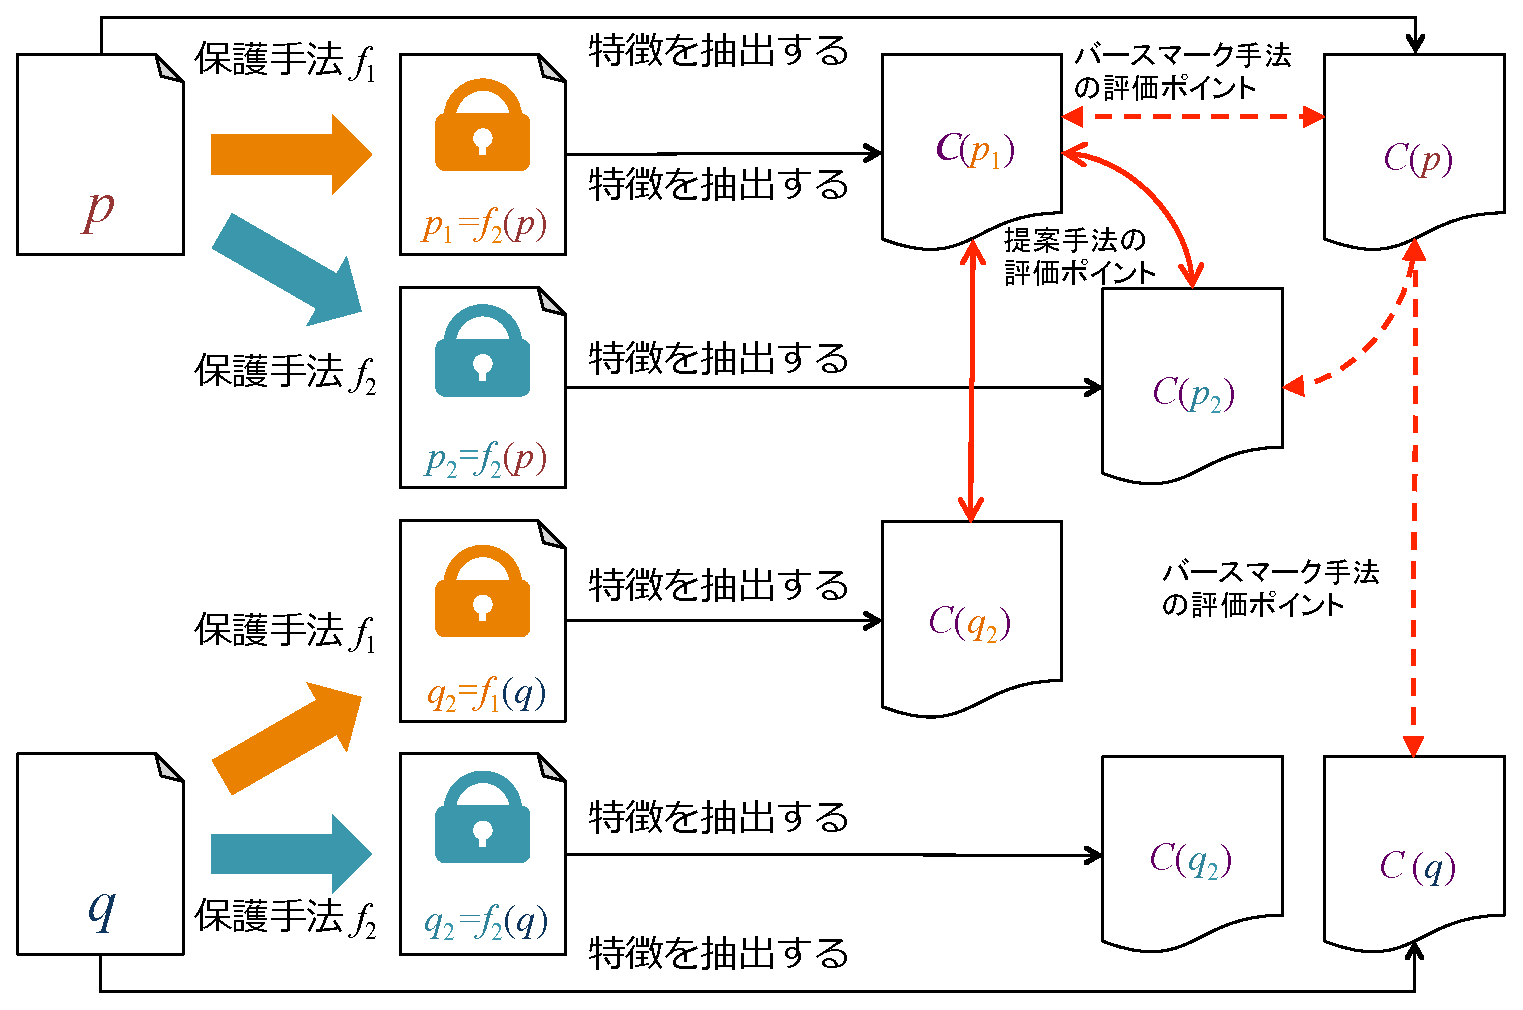
\includegraphics[width=0.78\textwidth]{images/key_idea}
  \caption{提案手法の模式図}\label{fig:keyidea}
\end{figure}

プログラム中の特徴で、他のプログラムと区別する手法に、バースマークが提
案されている\cite{tamada05ieice}。バースマークはプログラムが本来持って
いる特徴を抽出し、特徴同士を比較することで、盗用を発見する技術である。
本研究とは目的が異なるため、バースマークをそのままの適用はできないが、
比較方法をはじめとしたバースマーク手法の応用に期待できる。

神崎らはプログラムの不自然さを評価する手法を提案している
\cite{kanzaki14ipsj}。このプログラムはプログラムのオペコードから
$n$-gram を抽出し、生成確率を求めることで不自然さ評価を行っている。例えば、
松田らは、コード断片の不自然さを比較することで、保護手法の発見の困難さ
を評価している\cite{matsuda15ipsj}。


我々はこの手法に着目し、保護手法が特有の特徴を持つと仮定する。そして、
特有の特徴により、どのような保護手法が使われているかの特定を試みる。保
護手法が特定できれば、その保護手法に特化した攻撃手法や保護手法の理解に
よる攻撃が可能となる。逆に言えば、どのような保護手法かが特定できなけれ
ば、攻撃の足掛かりが掴めず、攻撃が困難になる。

図\ref{fig:keyidea}に提案手法の模式図を示す。提案手法もバースマークも、
保護されたプログラムから特徴を抽出するまでの処理は同じである一方で、評
価するポイントが異なる。図\ref{fig:keyidea}にあるように、プログラム$p$
を何らかの保護手法$f_1$と$f_2$で保護したプログラム$p_1=f_1(p)$,
$p_2=f_2(p)$を得る。そして、特徴抽出関数$\mathcal{C}$を用いて、$p,
p_1, p_2$から何らかの特徴 $\birth{p_1}, \birth{p_1}, \birth{p_2}$を得
る。
%
バースマーク技術での関心ごとは、図\ref{fig:keyidea}の点線での矢印で示
す部分であり、$\birth{p}$と$\birth{p_1}, \birth{p_2}$がどれくらい
似ているか、また、$\birth{p}$と$\birth{q}$がどのくらい違うかを評価
する。

提案手法での関心ごとは、図\ref{fig:keyidea}で実線矢印で示される部分で
ある。すなわち、異なる手法で保護した同じプログラムがどの程度違うのか
($\birth{p_1}$と$\birth{p_2}$)、同じ手法で保護した異なるプログラム
がどの程度似ているのか($\birth{p_1}$と$\birth{q_1}$)を比較する。

\section{特徴抽出法}\label{sect:artificiality}

抽出する特徴は、バースマークと似た手法になるものの、バースマークそのも
のは期待通りに働かない。なぜなら、異なるプログラム$p$と$q$を同じ手法
$f_1$で保護した場合、バースマークはプログラム自体が異なるため、異なっ
ているという結果を期待する($\birth{p_1} \neq \birth{q_1}$)。しかし、提
案手法は保護方法自体の特徴を取り出したいため、同じであるという結果を期
待する($\birth{p_1} \approx \birth{q_1}$)ためである。

そこで、神崎らの提案している不自然さ評価法に着目する
\cite{kanzaki14ipsj}。この手法は、オペコードの$n$-gramの珍しさを利用
するものである。保護手法の中には、絶対に実行されない箇所に本来は有りえ
ない順序の命令を挿入する場合や、既存の命令列を理解が困難なように珍しい
命令に置き換える場合がある。
%
そこで、珍しさを見ることによって、珍しい命令列であるか否かを判定できる。
このような珍しい命令列が保護手法の特徴であると言えるためである。生成確
率はパープレキシティを利用する\cite{gekka14scis}。パープレキシティとは
平均分岐数として知られ、言語としての複雑性を表す指標である。この値が小
さいほど、次に来る語が予測しやすいことを表す。そのため、値が小さいほど
自然であると言える。

一方で、保護手法の中ではコンパイラが出力した本来の命令を重複させる場合
もある。本来の命令は使用頻度の違いはあるものの、珍しいとは言い難い。そ
のため、生成頻度だけでは保護手法の特徴を見出せない可能性がある。そこで、
$n$-gramの頻度にも着目する。

以上のように、プログラムから命令の$n$-gramを抽出し、その珍しさ(パープ
  レキシティ)と頻度を保護手法の特徴とする。

\section{特徴の指標}\label{sect:index}

提案手法では、保護手法の適用前後でのオペコードの$n$-gramがどのように変化
したかで、保護手法の特徴を測定する。そこで、どの程度$n$-gramが変化した
かを次の4つの指標で測定する。まず、$p$を与えられたプログラム、$p_a$を
保護手法$f_a$により、$p$を保護したプログラムとする($p_a=f_a(p)$)。また、
$\mathcal{N}_n(p)$を$p$から抽出した$n$-gramの集合とし、そこから重複し
た$n$-gramを取り除いた集合を$\distinct{p}$とする。また、
$\mathcal{N}_n(p)$の頻度ベクトルを$\bm{p_a}=\{ (k^a_1, v^a_1), (k^a_2,
v^a_2), ..., (k^a_m, v^a_m) \}$とする。

このとき、$p$から$p_a$に変換して得られたプログラムがあったときに、次の4つの指標で保護手法の特徴を測定する。
\begin{enumerate}
\item 追加された$n$-gramの数 $M_a=$($\overline{\distinct{p}} \cap \distinct{p_a}$)、
\item 削除された$n$-gramの数 $M_d=$($\distinct{p} \cap \overline{\distinct{p_a}}$)、
\item $\distinct{p}$と$\distinct{p_a}$のJaccard係数 $M_j=$($\displaystyle
  \frac{|\distinct{p} \cap \distinct{p_a}|}{|\distinct{p} \cup
    \distinct{p_a}|}$)、
\item $\bm{p}$と$\bm{p_a}$のコサイン類似度 $M_c=$($\displaystyle
  \frac{\sum_{i=1}^{m} v_i v^a_i}{\sqrt{\sum_{i=1}^m v_i}
    \sqrt{\sum_{i=1}^m v^a_i}}$)
\end{enumerate}

これは、バースマーク手法における類似度計算に相当するものである。しかし、
本手法で着目すべきは、$p$と$p_1$もしくは、$p_1$と$q_1$であり、バースマー
クのように、一般的なプログラム同士の比較,例えば、$p$と$q$には着目しな
い。

\chapter{予備実験}

\section{概要}
%%始めのみ追加
評価実験を行う前に、予備実験を行う。
ここでは、提案手法により、本当に保護手法ごとに特徴が出ているのかを検出
することの確認を目的とする。そこで、Javaを対象とした難読化ツールを用い
て、実際にjarファイル$p, q, r$を難読化する。この難読化手法が$f_n$に相
当する。そして、難読化前後のjarファイルから特徴$\birth{p}, \birth{q},
\birth{r}, ..., \birth{p_n}, \birth{q_n}, \birth{r_n}$を抽出する。そし
て、得られた特徴をグラフにして、互いに比較する。

抽出する特徴は、第\ref{sect:artificiality}節で述べたようにオペコードの
$n$-gramを基本とし、そのパープレキシティと頻度を用いて比較を行う。
また、$n$は2, 3, 4, 5とした。

パープレキシティを導出するためにコーパスの構築が必要である。そのため、
The Apache Software Foundation\footnote{\url{http://www.apache.org/}}
で配布されているjarファイル 3,786 個を収集した。jarファイル内の総クラ
ス数は 660,465、総メソッド数は 4,272,567 である。

対象とするJarファイルは、
Javaバイトコード編集ライブラリ ASM
5.0.3\footnote{\url{http://asm.ow2.org}}、JVM言語の一つであるScala
2.11.6\footnote{\url{http://www.scala-lang.org}}、ユニットテストフレー
ムワークである JUnit 4.12\footnote{\url{http://junit.org}}を選択した。これ
らのjarファイルは全て Maven Central
Repository\footnote{\url{http://search.maven.org}} より取得した。

また、難読化ツールには、Allatori Java
Obfuscator\footnote{\url{http://www.allatori.com}}、
ProGuard\footnote{\url{http://proguard.sourceforge.net/}}、
yGuard\footnote{\url{https://www.yworks.com/en/products_yguard_about.html}}
の3つを選択した。

抽出する特徴は、第\ref{sect:artificiality}節で述べたようにオペコードの
$n$-gramを基本とし、そのパープレキシティと頻度を用いて比較を行う。
また、$n$は2, 3, 4, 5とした。

パープレキシティを導出するためにコーパスの構築が必要である。そのため、
The Apache Software Foundation\footnote{\url{http://www.apache.org/}}
で配布されているjarファイル 3,786 個を収集した。jarファイル内の総クラ
ス数は 660,465、総メソッド数は 4,272,567 である。

\begin{table}[t]
  \centering
  \caption{対象jarファイルの$n$-gramの種類数}\label{table:original}
  {\footnotesize
  \begin{tabular}{l|rrr}
    & JUnit & ASM All & Scala \\ \hline
File size & 315K & 2.5MB & 5.6MB\\ \hline
2-gram &   690 &  1,380 &  2,135 \\ 
3-gram & 2,173 &  5,000 &  8,328 \\
4-gram & 4,108 & 10,968 & 19,711 \\
5-gram & 5,730 & 17,465 & 32,793 
  \end{tabular}}
\end{table}

\begin{table}[t]
  \centering
  \caption{特徴の指標}\label{table:index}
{\footnotesize
  \begin{tabular}{ll|rrr||rrr}
    & & \multicolumn{3}{c|}{\textbf{2-gram}} & \multicolumn{3}{c}{\textbf{3-gram}} \\
    & & \rotatebox{45}{Allatori} & \rotatebox{45}{ProGuard} & \rotatebox{45}{yGuard} &
    \rotatebox{45}{Allatori} & \rotatebox{45}{ProGuard} & \rotatebox{45}{yGuard} \\ \hline
\multirow{4}{*}{\rotatebox{90}{\textbf{JUnit}}}
& 追加数($M_a$)       &   227 &    95 &     0 &   948 &   472 &     0 \\
& 削除数($M_d$)       &    28 &   100 &     3 &   308 &   494 &    10 \\
& Jaccard($M_j$)      & 0.722 & 0.752 & 0.996 & 0.598 & 0.635 & 0.995 \\
& $\cos$類似度($M_c$) & 0.929 & 0.962 & 1.000 & 0.763 & 0.912 & 1.000 \\ \hline
\multirow{4}{*}{\rotatebox{90}{\textbf{ASM All}}}
& 追加数($M_a$)       &   402 &   666 & 0     & 2,723 &   666 & 0 \\
& 削除数($M_d$)       &    51 &   312 & 0     &   787 &   312 & 0 \\
& Jaccard($M_j$)      &  0.746 & 0.827 & 1.000 &  0.546 & 0.827 & 1.000 \\
& $\cos$類似度($M_c$) & 0.871 & 0.950 & 1.000 & 0.676 & 0.950 & 1.000 \\ \hline
\multirow{4}{*}{\rotatebox{90}{\textbf{Scala}}}
& 追加数($M_a$)       &   415 & 1,749 & 0     & 3,095 & 1,749 & 0 \\
& 削除数($M_d$)       &    64 & 2,389 & 7     &   830 & 2,389 & 7 \\
& Jaccard($M_j$)      &  0.812 & 0.589 & 0.999 &  0.656 & 0.589 & 0.999 \\
& $\cos$類似度($M_c$) & 0.978 & 0.700 & 1.000 & 0.932 & 0.700 & 1.000 \\ \hline \hline
    & & \multicolumn{3}{c|}{\textbf{4-gram}} & \multicolumn{3}{c}{\textbf{5-gram}} \\ \hline
\multirow{4}{*}{\rotatebox{90}{\textbf{JUnit}}}
& 追加数($M_a$)       & 2,174 & 1,212 &     0 & 3,352 & 2,044 &     0 \\
& 削除数($M_d$)       & 1,095 & 1,280 &    27 & 2,188 & 2,191 &    37 \\
& Jaccard($M_j$)      & 0.480 & 0.532 & 0.994 & 0.390 & 0.455 & 0.994 \\
& $\cos$類似度($M_c$) & 0.539 & 0.842 & 0.999 & 0.424 & 0.787 & 0.999 \\ \hline
\multirow{4}{*}{\rotatebox{90}{\textbf{ASM All}}}
& 追加数($M_a$)       & 7,484 & 1,919 &     0 &13,135 & 3,621 & 0 \\
& 削除数($M_d$)       & 3,357 & 1,114 &     0 & 7,897 & 2,586 & 0 \\
& Jaccard($M_j$)      &  0.412 & 0.765 & 1.000 & 0.313 & 0.706 & 1.000 \\
& $\cos$類似度($M_c$) & 0.448 & 0.908 & 1.000 & 0.308 & 0.844 & 1.000 \\ \hline
\multirow{4}{*}{\rotatebox{90}{\textbf{Scala}}}
& 追加数($M_a$)       &  9,385 & 6,275 &    0 &17,697 &12,668 &     0 \\
& 削除数($M_d$)       &  4,305 & 7,992 &   54 &10,857 &16,515 &   132 \\
& Jaccard($M_j$)      &  0.530 & 0.451 & 0.997 & 0.434 & 0.358 & 0.996 \\
& $\cos$類似度($M_c$) & 0.816 & 0.629 & 1.000 & 0.532 & 0.678 & 1.000
  \end{tabular}}
\end{table}

\section{提案指標による比較}

まず、対象となるjarファイルのファイルサイズと、取り出した$n$-gramの種類
数を調査した。結果を表\ref{table:original}に示す。ファイルサイズに比例
して、そして、$n$にも比例して$n$-gramの種類数が増加していることがわか
る。
%
次に、それらのjarファイルを3つの難読化ツールにかけ、それぞれ3つの保護
されたプログラムを得る。元のプログラムと難読化されたプログラムの計4種
類のプログラムから、$n$-gramを抽出し、第\ref{sect:index}節で述べた指標
を計算した結果を表\ref{table:index}に示す。

表\ref{table:index}を見ると、yGuardはオペコードの$n$-gramをほとんど変
化させず、提案手法では、特徴を取り出せないことがわかる。
%
一方、AllatoriとProGuardは、積極的にオペコードを変更している。Allatori
は多くのオペコードを追加することで、難読化を実現し、ProGuardは既存の命
令を変更することが、オペコードの$n$-gramの削除数に繋がっていると考えら
れる。

\section{オペコードの$n$-gramのヒストグラム}

ここでは、難読化前後の各プログラムのオペコードから、3-gramを抽出した。
そのヒストグラムを図\ref{fig:scala-3gram-histogram}に示す。全てのグラ
フの横軸は、難読化前後で得られたプログラムそれぞれから抽出した$3$-gram
集合の和集合\footnote{ $\distinctnnn{p} \cup \distinctnnn{p_{\rm
      Allatori}} \cup \distinctnnn{p_{\rm ProGuard} \cup
    \distinctnnn{p_{\rm yGuard}}}$}であり、縦軸が対応する$n$-gramの頻
度を対数で表している。図\ref{fig:scala-3gram-histogram}に示す4つのグラ
フの横軸はすべて同じであり、頻度でソートしている。

図を見ると、AllatoriやProGuardで難読化したとき、オリジナルとは異なると
ころにも山ができている。これは、オリジナルにない命令が、難読化後のプロ
グラムに大量に追加されていることを示している。AllatoriとProGuardで同じ
3-gramが追加されている場合、異なる3-gramが追加されている場合がある。追
加された3-gramは最大で1,000程度存在することもわかる。

一方で、yGuardのヒストグラムは、表\ref{table:index}からもわかるように、
オリジナルと大きく変化しないため、提案手法による識別は困難であると言える。

\begin{figure}[b]
  \centering
  \subfigure[オリジナル]{
    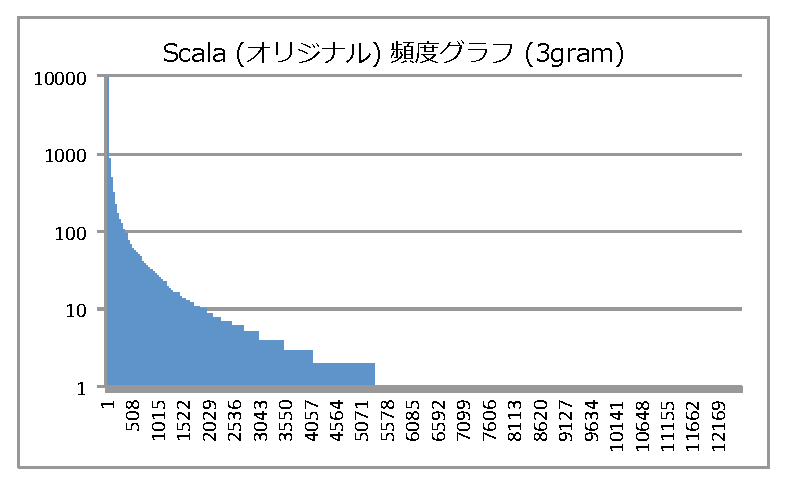
\includegraphics[clip,width=0.48\columnwidth]{images/scala-3gram-original-histogram}
    \label{fig:scala-3gram-original-histogram}
  }%
  \subfigure[Allatori]{
    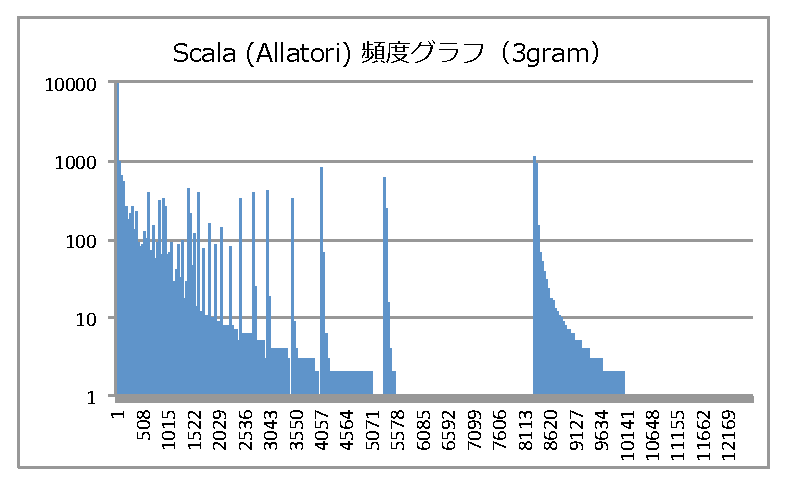
\includegraphics[clip,width=0.48\columnwidth]{images/scala-3gram-allatori-histogram}
    \label{fig:scala-3gram-allatori-histogram}
  }
  \subfigure[yGuard]{
    \includegraphics[clip,width=0.48\columnwidth]{images/scala-3gram-yGuard-histogram}
    \label{fig:scala-3gram-yguard-histogram}
  }%
  \subfigure[ProGuard]{
    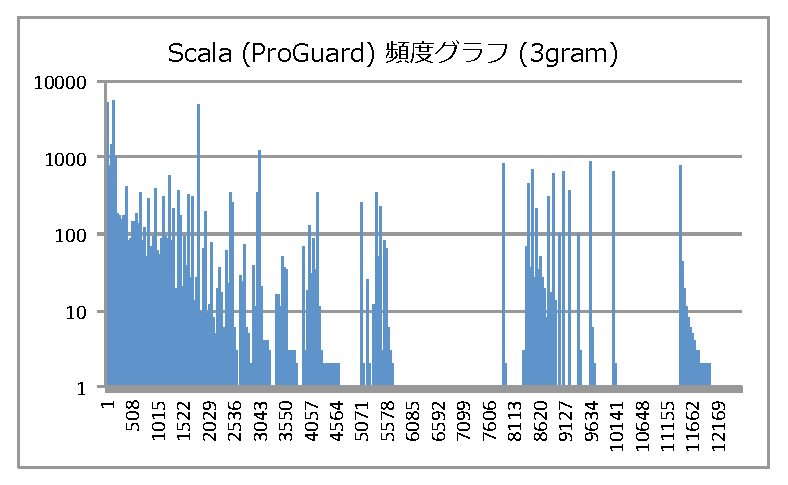
\includegraphics[clip,width=0.48\columnwidth]{images/scala-3gram-proguard-histogram}
    \label{fig:scala-3gram-proguard-histogram}
  }
  \caption{Scalaのオペコードの$3$-gram ヒストグラム(頻度でソート)}\label{fig:scala-3gram-histogram}
\end{figure}

また、ASMの難読化前後で$5$-gramを抽出した場合の結果を図
\ref{fig:asm-5gram-histogram}に示す。図\ref{fig:asm-5gram-histogram}で
は、オペコードのソート方法を頻度からパープレキシティに変更している。な
お、図\ref{fig:asm-5gram-perplexity}にパープレキシティのグラフを示して
いる。
%
これらのグラフから、Allatori は、パープレキシティが高い$5$-gramであっ
ても、頻度が下がっていないものの、オリジナル、yGuard、ProGuardではパー
プレキシティが高いものの頻度が低くなっていることがわかる。

\begin{figure}[b]
  \subfigure[パープレキシティ]{
    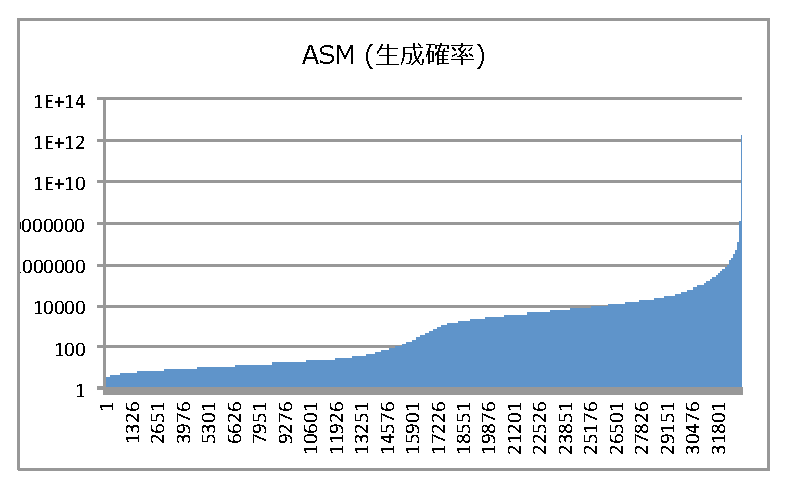
\includegraphics[clip,width=0.48\columnwidth]{images/asm-5gram-perplexity}
    \label{fig:asm-5gram-perplexity}
  }
  \centering
  \subfigure[オリジナル]{
    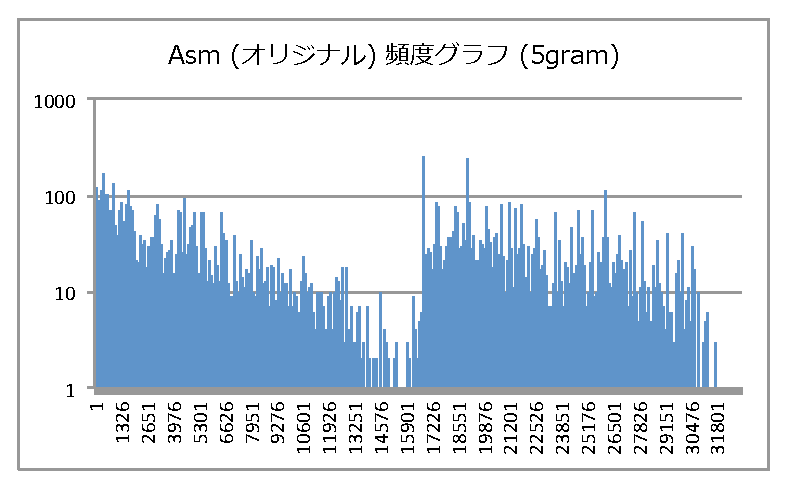
\includegraphics[clip,width=0.48\columnwidth]{images/asm-5gram-original-histogram}
    \label{fig:asm-5gram-original-histogram}
  }%
  \subfigure[Allatori]{
    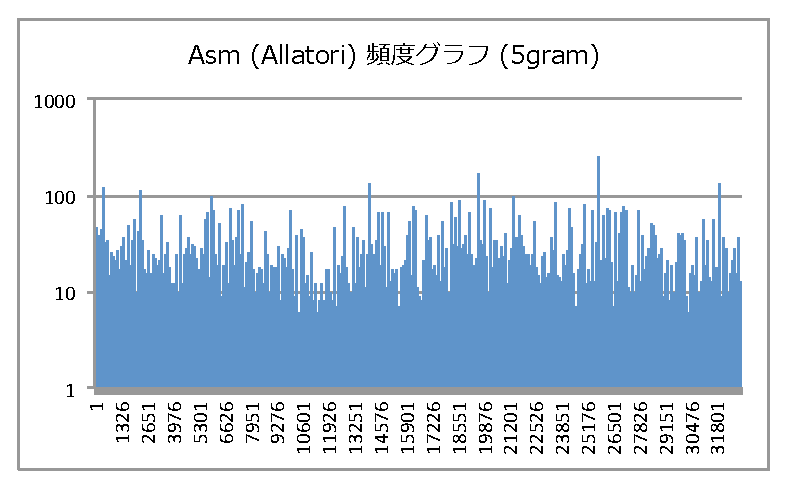
\includegraphics[clip,width=0.48\columnwidth]{images/asm-5gram-allatori-histogram}
    \label{fig:asm-5gram-allatori-histogram}
  }
  \subfigure[yGuard]{
    \includegraphics[clip,width=0.48\columnwidth]{images/asm-5gram-yGuard-histogram}
    \label{fig:asm-5gram-yguard-histogram}
  }%
  \subfigure[ProGuard]{
    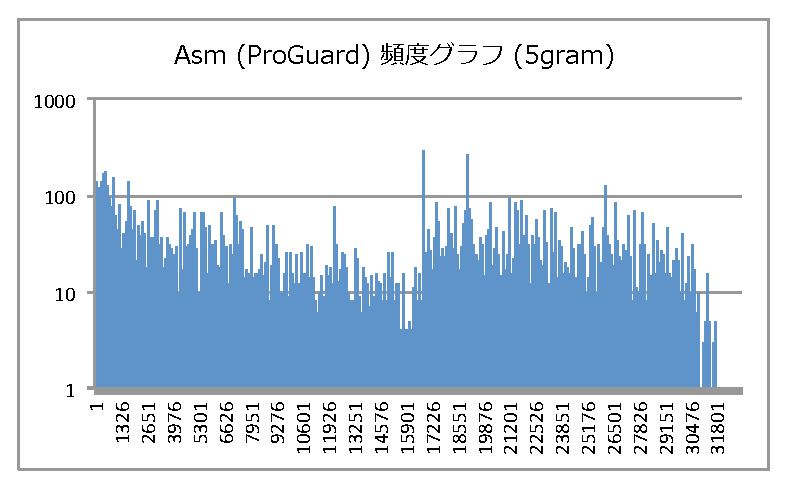
\includegraphics[clip,width=0.48\columnwidth]{images/asm-5gram-proguard-histogram}
    \label{fig:asm-5gram-proguard-histogram}
  }
  \caption{ASMのオペコードの$5$-gram ヒストグラム(パープレキシティでソート)}\label{fig:asm-5gram-histogram}
\end{figure}


\section{オペコードの$n$-gramのパープレキシティ}

\begin{table*}[t]
  \centering
%   \caption{Scalaの難読化前後のオペコードの5-gram(上位5位)}\label{table:5gram}
%   {\footnotesize
%   \begin{tabular}{lc|l|rrrr|r}
%     & 順位 & 5-gram & オリジナル & Allatori & ProGuard & yGuard & パープレキシティ \\ \hline
% \multirow{5}{*}{\rotatebox{90}{オリジナル}}
% & 1 & \verb!aload aload aload invokestatic areturn            ! & 2,293 & 2,293 &   995 & 2,293 & 6.3 \\
% & 2 & \verb!aload instanceofInsn ifeq aload checkcast         ! & 1,342 &   257 & 1,097 & 1,342 & 1664.7 \\
% & 3 & \verb!aload invokestatic aload invokestatic aload       ! & 1,276 &     6 &    53 & 1,276 & 6.6\\
% & 4 & \verb!aload aload putfield aload invokespecial          ! & 1,215 &       &   771 & 1,215 & 4538.7\\
% & 5 & \verb!invokestatic aload invokestatic aload invokestatic! & 1,146 &     6 &     6 & 1,146 & 499.5 \\ \hline
% \multirow{5}{*}{\rotatebox{90}{Allatori}}
% & 1 & \verb!aload aload aload invokestatic areturn  ! & 2,293 & 2,293 &   995 & 2,293 & 6.3 \\
% & 2 & \verb!instanceofInsn aload swap ifeq checkcast! &       &   965 &       &       & $4.7 \times 10^6$\\
% & 3 & \verb!aload aload aload aload aload           ! &   869 &   847 &   244 &   869 & 4.7 \\
% & 4 & \verb!aload swap ifeq checkcast aload         ! &       &   815 &       &       & 147,517 \\
% & 5 & \verb!swap ifeq checkcast aload invokestatic  ! &       &   810 &       &       & 149,657 \\ \hline
% \multirow{5}{*}{\rotatebox{90}{ProGuard}}
% & 1 & \verb!aload instanceofInsn ifeq aload checkcast! & 1,342 &   257 & 1,097 & 1,342 & 1664.7\\
% & 2 & \verb!aload dup astore getfield aload          ! &       &       & 1,049 &       & 36.6  \\
% & 3 & \verb!aload aload aload invokestatic areturn   ! & 2,293 & 2,293 &   995 & 2,293 & 6.3   \\
% & 4 & \verb!gotoInsn aload instanceofInsn ifeq aload ! & 1,063 &    36 &   945 & 1,063 & 3.1   \\
% & 5 & \verb!instanceofInsn ifeq aload checkcast aload! &   814 &    13 &   794 &   814 & 2.3
%   \end{tabular}}
  \caption{Scalaの難読化前後のオペコードの5-gram(上位5位)}\label{table:5gram}
  {\footnotesize
  \begin{tabular}{lc|l}
    & 順位 & 5-gram \\ \hline
\multirow{5}{*}{\rotatebox{90}{オリジナル}}
& 1 & \verb!aload aload aload invokestatic areturn            ! \\
& 2 & \verb!aload instanceofInsn ifeq aload checkcast         ! \\
& 3 & \verb!aload invokestatic aload invokestatic aload       ! \\
& 4 & \verb!aload aload putfield aload invokespecial          ! \\
& 5 & \verb!invokestatic aload invokestatic aload invokestatic! \\ \hline
\multirow{5}{*}{\rotatebox{90}{Allatori}}
& 1 & \verb!aload aload aload invokestatic areturn  ! \\
& 2 & \verb!instanceofInsn aload swap ifeq checkcast! \\
& 3 & \verb!aload aload aload aload aload           ! \\
& 4 & \verb!aload swap ifeq checkcast aload         ! \\
& 5 & \verb!swap ifeq checkcast aload invokestatic  ! \\ \hline
\multirow{5}{*}{\rotatebox{90}{ProGuard}}
& 1 & \verb!aload instanceofInsn ifeq aload checkcast! \\
& 2 & \verb!aload dup astore getfield aload          ! \\
& 3 & \verb!aload aload aload invokestatic areturn   ! \\
& 4 & \verb!gotoInsn aload instanceofInsn ifeq aload ! \\
& 5 & \verb!instanceofInsn ifeq aload checkcast aload!
  \end{tabular}}
  \vfill
  \caption{Scalaの難読化前後のオペコードの5-gramの頻度(上位5位)}\label{table:5gram_f}
  {\footnotesize
  \begin{tabular}{lc|rrrr|r}
    & 順位 & オリジナル & Allatori & ProGuard & yGuard & PPL \\ \hline
    \multirow{5}{*}{\rotatebox{90}{オリジナル}}
& 1 & 2,293 & 2,293 &   995 & 2,293 &    6.3 \\
& 2 & 1,342 &   257 & 1,097 & 1,342 & 1664.7 \\
& 3 & 1,276 &     6 &    53 & 1,276 &    6.6 \\
& 4 & 1,215 &       &   771 & 1,215 & 4538.7 \\
& 5 & 1,146 &     6 &     6 & 1,146 &  499.5 \\ \hline
\multirow{5}{*}{\rotatebox{90}{Allatori}}
& 1 & 2,293 & 2,293 &   995 & 2,293 &         6.3 \\
& 2 &       &   965 &       &       & 4,700,000\\
& 3 &   869 &   847 &   244 &   869 &         4.7 \\
& 4 &       &   815 &       &       &   147,517 \\
& 5 &       &   810 &       &       &   149,657 \\ \hline
\multirow{5}{*}{\rotatebox{90}{ProGuard}}
& 1 & 1,342 &   257 & 1,097 & 1,342 & 1664.7 \\
& 2 &       &       & 1,049 &       &   36.6 \\
& 3 & 2,293 & 2,293 &   995 & 2,293 &    6.3 \\
& 4 & 1,063 &    36 &   945 & 1,063 &    3.1 \\
& 5 &   814 &    13 &   794 &   814 &    2.3
  \end{tabular}}
\end{table*}

図\ref{fig:scala-perplexity}にScalaでの$n$-gramのパープレキシティを示
す。横軸は、図\ref{fig:scala-3gram-histogram}と同じように、得られた
$n$-gramであり、縦軸がそのパープレキシティを対数で表したものである。横軸の
$n$-gram はグラフごとに異なっているものの、すべて当該項目で抽出できた
$n$-gramの和集合である。また、頻度によってソートされている。
%
いずれのグラフも、左側は同じような値が続き、中央左で値が大きくなっている、
%
これは、パープレキシティは、低いほど自然であることを表していることから、
オリジナルで得られた$n$-gramは珍しい命令の並びではなく、ありふれた命令
の並びであることを示す。そして、中央左で値が高くなっている部分では、
AllatoriやProGuardで新たに追加された$n$-gramが示されており、この命令の
並びはありふれた並びではないことがわかる。

\begin{figure}[b]
  \centering
  \subfigure[2gram]{
    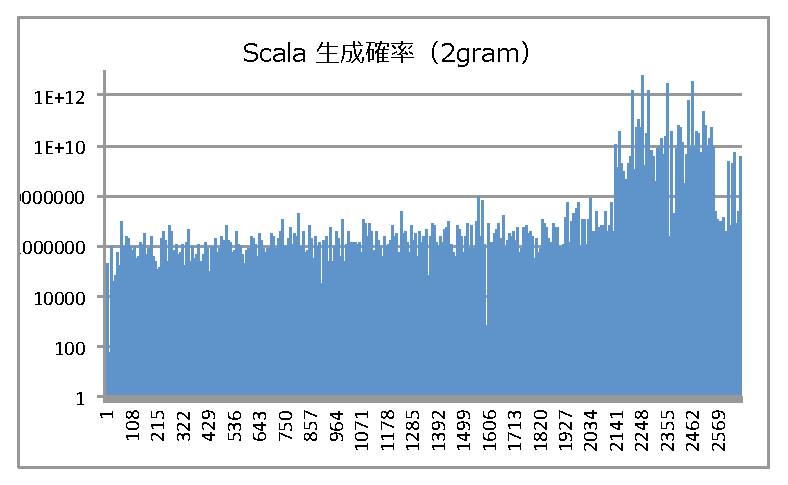
\includegraphics[clip,width=0.48\columnwidth]{images/scala-2gram-perplexity}
    \label{fig:scala-2gram-ppl}
  }%
  \subfigure[3gram]{
    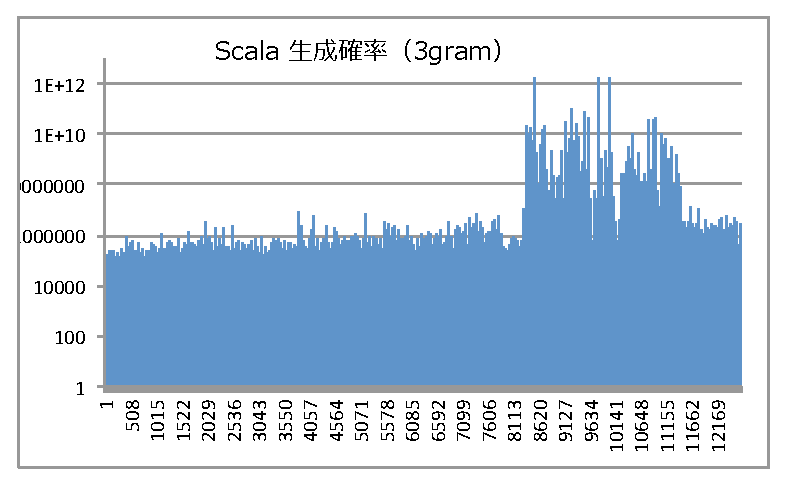
\includegraphics[clip,width=0.48\columnwidth]{images/scala-3gram-perplexity}
    \label{fig:scala-3gram-ppl}
  }
  \subfigure[4gram]{
    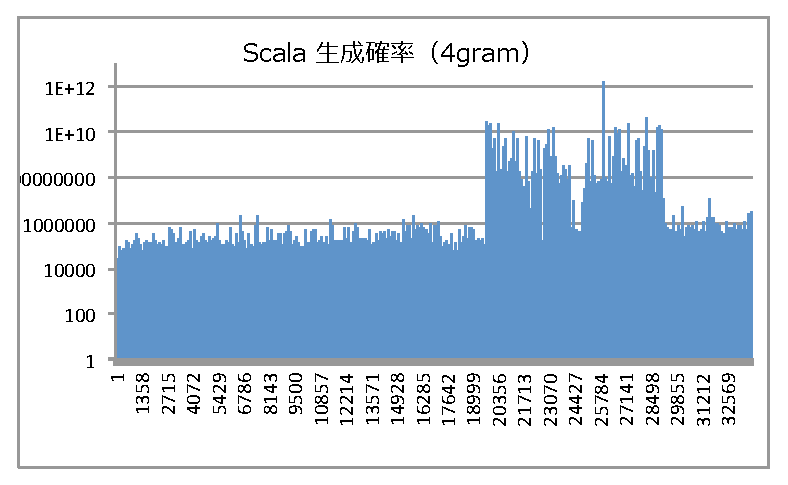
\includegraphics[clip,width=0.48\columnwidth]{images/scala-4gram-perplexity}
    \label{fig:scala-4gram-ppl}
  }%
  \subfigure[5gram]{
    \includegraphics[clip,width=0.48\columnwidth]{images/scala-5gram-perplexity}
    \label{fig:scala-5gram-ppl}
  }
  \caption{Scalaのオペコードの$n$-gram 生成確率}\label{fig:scala-perplexity}
\end{figure}

\section{抽出された$n$-gramの分析}

ここでは、実際に抽出された$n$-gramから、どのような命令であるのかを確認
する。$n$が大きいほど、どのようなコードであるかの理解が容易であるため、
$n=5$の場合を確認する。
%
表\ref{table:5gram},表\ref{table:5gram_f}に、Scalaの難読化前、Allatori、ProGuardで難読化した
それぞれのプログラムから抽出した5-gramの頻度上位5つを示している。命令
列の右側に、当該5-gramの難読化前後での頻度、パープレキシティを示している。

オリジナルの5-gramを確認する。1位は、staticメソッドの呼び出し後、値を
返す命令の並び、2位は、instanceof で値を比較したあと、キャストしている。
3位, 4位, 5位もメソッド呼び出しを中心とした命令の並びであり、ありふれ
た命令列である。パープレキシティを見ると、1, 3, 5位の命令列は低いもの
の、2, 4位の命令列は、若干高くなっている。しかし、4位の命令であっても、
ローカル変数をフィールドに代入後、privateメソッドの呼び出しと、ソース
コードに素直に変換できる単純な命令の並びである。そのため、ありふれた命
令であると言える。

一方、Allatori、ProGuard にしか出現していない命令の並びを見てみると、
命令の順序を入れ替えた上で、\texttt{swap}でスタックの順序も入れ替えて
いるものが見られる。
%
例えば、Allatori の2位、4位、5位の命令列は、他のパープレキシティに比べ
ても、非常に高くなっている。しかし、オリジナルの2位の命令列を元にして
いると考えられる。なぜなら、Allatoriの2, 4, 5位の命令列は、
\texttt{instanceofInsn aload swap ifeq checkcast aload invokestatic}と
いう7つの命令から抽出されたと考えられる、これは、オリジナル2位の
\texttt{aload instanceofInsn ifeq aload checkcast}の3番目に
\texttt{swap}命令を挿入し、その前の2つの命令の順序を入れ替えたものに相
当するためである。

また、ProGuard の2位の命令列は、ここでは、ProGuardにしか現れていないも
のの、パープレキシティを見ると、それほど珍しくない命令でもある。この5
つの命令列から取り出した4-gramは、オリジナルの4gramにも含まれているこ
とが確認できた。

このことから、Allatoriは命令の並び中に \texttt{swap} 命令を入れ、命令
の順序を入れ替えることで難読化を実現していると考えられる。Allatoriのみ
に追加された5-gramを調査したところ、概ねそのような変換が施されていると
推測できた。その結果、珍しい命令列が抽出されることになり、Allatoriの特
徴が掴めたことになる。

一方で、ProGuardは、ProGuardのみで抽出できた頻度が300以上の$5$-gramを確
認したところ、著しく珍しいと言える5-gramは見つからなかった。そのため、
命令列自体を変更しているものの、ProGuardならではの特徴を抽出するには至
らなかった。そのため、ProGuardならではの特徴を掴むには、他のアプローチ
に取り組む必要がある。

%%追加
予備実験では、不自然さ評価に着目して、適用された保護手法の特定に取り組んだ。
実際のプログラムに、3種類の保護手法を適用し、不自然さ評価の指標を抽出した。
その結果、保護手法の1つであるAllatoriは提案手法により、識別の可能性が見られた。
一方で、他の保護手法である、ProGuardやyGuardは難読化前のプログラムと、
オペコードに大きな違いが見られなかった。

\chapter{評価実験}

\section{概要}

%%変更あり

予備実験により保護手法には何らかの特徴があることが判明した。
ここでは、抽出した特徴から保護手法を決定づけられるかを目的とする。

抽出する特徴は、第\ref{sect:artificiality}節で述べたようにオペコードの
$n$-gramを基本とし、そのパープレキシティと頻度を用いて比較を行う。対象
とするJarファイルは表\ref{table:jars}に、難読化ツールは表
\ref{table:tools}に記す。

\begin{table}[t]
  \centering
  \footnotesize{
    \caption{利用したJarファイル一覧}\label{table:jars}
  \begin{tabular}{l|r||l|r||l|r}
    Product & Version & Product & Version & Products & Version \\ \hline
    ASM       & 3.3.1 & FakeHack  & 1.0 &JCalendar & 1.3.3   \\
    Jhstop    & 0.0.1 & Jwhich    & 1.0   & Robocode-setup & 1.6.0.1 
  \end{tabular}
  \caption{利用した難読化ツール}\label{table:tools}
  \begin{tabular}{ll|l}
      Tools & Abbr. & Overview \\ \hline
      Allatori Java Obfuscator & ALL & 商用の難読化ツール \\ \hline
      ProGurad                 & PG & OSSの難読化ツール \\ \hline
      Sandmark                 & & 研究用の難読化ツール \\
      \hspace{0.2cm} Duplication registers & DR & 代入を重複させる。\\
      \hspace{0.2cm} Merge local integers & MLI & 2つのint変数をlongに収める。\\
      \hspace{0.2cm} Irreducibility       & IRR & 制御フローを複雑にする。\\
  \end{tabular}}
\end{table}


その解析結果をもとに、不明な難読化手法の解析を行う。
初めに、未知のプロダクトを評価実験で扱う
5つの難読化手法 (表\ref{table:tools}) をランダムに選択し、難読化する。
その後、どの難読化手法が使われているかを検証する。
次に、既知のプロダクト (表\ref{table:jars}) を未知の難読化手法で難読化する。
その後、どの難読化手法が使われているかを検証する。
未知のプロダクトとしてJUnit 3.7を使用した。
%このプロダクトはユニットテストフレームワークである。
また、未知の難読化手法としてSandmarkのSimple Opaque Predicates (SOP) を使用した。

\section{$n$-gramの分析}

ここでは、それぞれの難読化手法を頻度とパープレキシティを参考に$n$-gramの命令列を解析した。
%それぞれの頻度順でソートしたASMをの表\ref{table:asm}に、
%オリジナル順にソートしたグラフ\ref{fig:graph}を付録に記す。

解析した結果、難読化手法の保護前後で違った命令列がみられた。
また、追加された命令列はパープレキシティの値が高く、珍しい命令列であることがわかった。
これらのデータから追加された命令列を難読化手法の特徴とし、その特徴を表\ref{table:features}に記す。

\begin{table}[t]
  \centering
  \footnotesize{
    \caption{ツールごとの特徴}\label{table:features}
  \begin{tabular}{l|l}
    ツール              & 特徴 \\ \hline
    ALL & オリジナルの命令列を\texttt{swap}命令で入れ替える \\
    PG  & オリジナルと変化なし \\
    DR  & \texttt{istore}命令を2回続けて実行する \\
    MLI & \texttt{dup2x2 lxor}を連続して実行する \\
    IRR & \texttt{nop}命令がある \\
  \end{tabular}}
\end{table}

\section{既知の難読化手法の特定}\label{sect:5gram_analysis}

ここでは、未知のプロダクトを表\ref{table:tools}のいずれかを用いて難読
化し、どの難読化手法が使われているかを検証する。難読化適用前の
$n$-gramに出現していない$n$-gramを調査した。その結果のうち、高頻度の
$n$-gramを5つ、表\ref{table:junit}に記す。

\begin{table}[t]
  \centering
  \footnotesize{
    \caption{JUnit (5-gram)の命令列}\label{table:junit}
  \begin{tabular}{l|r|r}
    命令列 & 頻度 & PPL\\ \hline
 %   \multicolumn{1}{p{1cm}}{ORI} & 
 %   \multicolumn{1}{p{1cm}}{ALL} & 
 %   \multicolumn{1}{p{1cm}}{DR} & 
 %   \multicolumn{1}{p{1cm}}{IRR} & 
 %   \multicolumn{1}{p{1cm}}{MLI} & 
 %   \multicolumn{1}{p{1cm}}{PG} & 
 %   \multicolumn{1}{p{1cm}}{PPL} \\ \hline
    \texttt{dup2x2 lxor lconst\_1 lneg bipush}   & 16 & 11.30E+05 \\
    \texttt{lload dup2x2 lxor lconst\_1 lneg}    & 16 &   5.37E+05 \\
    \texttt{bipush lushr land lxor lstore}       &  9 &   0.52E+05 \\
    \texttt{lconst\_1 leng bipush lushr land}    &  9 &   0.96E+05 \\
    \texttt{lneg bipush lushr land lxor}         &  9 &  1.37E+05 \\
  \end{tabular}}
\end{table}

表\ref{table:junit}をみると、命令列には、\texttt{dup2x2 lxor}といった
パープレキシティの値が高い命令列を呼び出している。その命令列を特徴とし、
5つのツールの特徴(表\ref{table:features})と比較する。その結果、適用さ
れている難読化手法の特徴とMLI手法の特徴が当てはまる。

\section{未知の難読化手法の特定}

ここでは、既知のプロダクトを未知の難読化手法で難読化を行い、どの難読化
手法が使われているかを検証する。難読化適用前の$n$-gramに出現していない
$n$-gramを調査した。その結果のうち、高頻度の$n$-gramを5つ、表
\ref{table:jhstop}に記す。

\begin{table}[t]
  \centering
  \footnotesize{
    \caption{Jhstop (5-gram)の命令列}\label{table:jhstop}
  \begin{tabular}{l|r|r}
   命令列 & 頻度 & PPL\\ \hline
 %   \multicolumn{1}{p{1cm}}{ORI} & 
 %   \multicolumn{1}{p{1cm}}{ALL} & 
 %   \multicolumn{1}{p{1cm}}{DR} & 
 %   \multicolumn{1}{p{1cm}}{IRR} & 
 %   \multicolumn{1}{p{1cm}}{MLI} & 
 %   \multicolumn{1}{p{1cm}}{PG} & 
 %   \multicolumn{1}{p{1cm}}{PPL} \\ \hline  
    \texttt{irem iconst\_0 if\_icmpne aload getfield} & 15 &   0.15E+05 \\
    \texttt{dup dup dup imul imul}                    & 14 &  42.40E+05 \\
    \texttt{dup dup imul imul isub}                   & 14 &   8.74E+05 \\
    \texttt{dup imul imul isub iconst\_3}             & 14 &   3.49E+05 \\
    \texttt{iload dup dup dup imul}                   & 14 & 101.00E+05 \\
    \end{tabular}}
\end{table}

表\ref{table:jhstop}をみると、パープレキシティの高い命令列であり、
\texttt{dup}, \texttt{imul}命令を連続で呼び出している。その命令列を特
徴とし、5つのツールの特徴(表\ref{table:features})と比較する。その結果、
未知の難読化手法の特徴は、解析したどの特徴にも当てはまらなかった。

次に、異なるプロダクトを未知の難読化手法で難読化し、それぞれの特徴を比較する。
その結果、同様の特徴が検出されたため、未知の難読化手法がSOP手法だとわかった。

\chapter{まとめ}

本稿では不自然さ評価に着目して、適用された保護手法の特定に取り組んだ。
実際のプログラムに、保護手法を適用し、$n$-gramの命令列を頻度やパープレキシティ
を基に、特徴を抽出した。その結果をもとに不明な難読化の解析を行った。
今回の評価実験では、既知の難読化は特定しやすいが、
未知の難読化の特定は難しい。
この解決策として、難読化手法の特徴を増やすことである。
特徴を増やすことで未知の難読化手法に対応できる。


 \bibliographystyle{csg-thesis}
 \bibliography{sagisaka}

\appendix
\chapter{5-gramの命令列}
表\ref{table:asm},表\ref{table:asm_f}に示す命令列は第\ref{sect:5gram_analysis}節で解析をしたデータである。難読化を適用する前と、それぞれの難読化を適用した後の命令列を頻度順でソートを行った。

\begin{table*}[t]
  \centering
  \caption{ASMの難読化前後のオペコードの5-gram(上位5位)}\label{table:asm}
  {\footnotesize
  \begin{tabular}{lc|l}
    & 順位 & 5-gram \\ \hline
\multirow{5}{*}{\rotatebox{90}{オリジナル}}
& 1 & \verb!<code> <code> <code> <code> aload      ! \\
& 2 & \verb!<code> <code> <code> aload getfield    ! \\
& 3 & \verb!<code> <code> <code> aload dup         ! \\
& 4 & \verb!aload dup getfield swap getfield       ! \\
& 5 & \verb!aload getfield ldc invokestatic invokevirtual! \\ \hline
\multirow{5}{*}{\rotatebox{90}{ALL}}
& 1 & \verb!dup2X2 lxor lconst1 lneg bipush  ! \\
& 2 & \verb!lload dup2X2 lxor lconst1 lneg   ! \\
& 3 & \verb!aload lload bipush lshr l2i           ! \\
& 4 & \verb!<code> <code> <code> <code> aload        ! \\
& 5 & \verb!bipush lushr land lxor lstore  ! \\ \hline
\multirow{5}{*}{\rotatebox{90}{DR}}
& 1 & \verb!<code> <code> <code> <code> aload  ! \\
& 2 & \verb!<code> <code> <code> aload getfield! \\
& 3 & \verb!iconst1 isub istore iload iload         ! \\
& 4 & \verb!istore iload aload arraylength ifcmpge        ! \\
& 5 & \verb!iconst0 dup istore istore iload  ! \\ \hline
\multirow{5}{*}{\rotatebox{90}{IRR}}
& 1 & \verb!aload aload aload invokestatic areturn  ! \\
& 2 & \verb!instanceofInsn aload swap ifeq checkcast! \\
& 3 & \verb!aload aload aload aload aload           ! \\
& 4 & \verb!iload iconst1 isub istore iload        ! \\
& 5 & \verb!i2l iconst0 i2l lcmp iconst1 ! \\ \hline
\multirow{5}{*}{\rotatebox{90}{MLI}}
& 1 & \verb!dup2X2 lxor lconst1 lneg bipush  ! \\
& 2 & \verb!lload dup2X2 lxor lconst1 lneg! \\
& 3 & \verb!aload lload bipush lshr l2i         ! \\
& 4 & \verb!<code> <code> <code> <code> aload        ! \\
& 5 & \verb!bipush lushr land lxor lstore  ! \\ \hline
\multirow{5}{*}{\rotatebox{90}{PG}}
& 1 & \verb!aload instanceofInsn ifeq aload checkcast! \\
& 2 & \verb!aload dup astore getfield aload          ! \\
& 3 & \verb!aload aload aload invokestatic areturn   ! \\
& 4 & \verb!gotoInsn aload instanceofInsn ifeq aload ! \\
& 5 & \verb!instanceofInsn ifeq aload checkcast aload!
  \end{tabular}}
\end{table*}

縦軸は頻度、横軸はオリジナルの頻度順にソートしたグラフ\ref{fig:graph}である。
このグラフから保護手法の前後に命令列が追加されているのがわかる。

\begin{table*}[t]
 \centering
  \caption{ASMの難読化前後のオペコードの5-gramの頻度(上位5位)}\label{table:asm_f}
  {\footnotesize
  \begin{tabular}{lc|rrrrrr|r}
  %  & 順位 & オリジナル & ALL & DR & IRR & MLI & PG & PPL \\ \hline
                                  &
    \multicolumn{1}{p{1cm}}{順位} & 
    \multicolumn{1}{p{1cm}}{ORI}  & 
    \multicolumn{1}{p{1cm}}{ALL}  & 
    \multicolumn{1}{p{1cm}}{DR}   & 
    \multicolumn{1}{p{1cm}}{IRR}  & 
    \multicolumn{1}{p{1cm}}{MLI}  & 
    \multicolumn{1}{p{1cm}}{PG}   & 
    \multicolumn{1}{p{1cm}}{PPL} \\ \hline
\multirow{5}{*}{\rotatebox{90}{オリジナル}}
& 1 & 219 & 206 & 219 & 219 & 193 & 219 & 61.19 \\
& 2 & 122 &  93 & 122 & 122 & 108 & 122 & 659.44 \\
& 3 & 37  &  22 &  37 &  36 &  37 &  37 & 2478.75 \\
& 4 & 32  &   1 &  32 &  31 &  19 &  32 & 2305.93 \\
& 5 & 30  &     &  30 &  30 &  30 &  30 & 7249.22 \\ \hline
\multirow{5}{*}{\rotatebox{90}{ALL}}
& 1 & 219 & 206 & 219 & 219 & 193 & 219 & 61.19 \\
& 2 & 122 &  93 & 122 & 122 & 108 & 122 & 659.44 \\
& 3 & 7   &  52 &   7 &     &     &     & 45551.95 \\
& 4 &     &  39 &     &     &     &     & 319006.00 \\
& 5 &     &  32 &     &     &     &     & 5954.31 \\ \hline
\multirow{5}{*}{\rotatebox{90}{DR}}
& 1 & 219 & 206 & 219 & 219 & 193 & 219 & 61.19 \\
& 2 & 122 &  93 & 122 & 122 & 108 & 122 & 659.44 \\
& 3 & 37  &  22 &  37 &  36 &  37 &  37 & 2478.75 \\
& 4 & 32  &   1 &  32 &  31 &  19 &  32 & 2305.93 \\
& 5 &     &     &  30 &     &     &     & 10835.90\\ \hline
\multirow{5}{*}{\rotatebox{90}{IRR}}
& 1 & 219 & 206 & 219 & 219 & 193 & 219 & 61.19 \\
& 2 & 122 &  93 & 122 & 122 & 108 & 122 & 659.44 \\
& 3 &   1 &     &   1 &  72 &   1 &   1 & 40200.30 \\
& 4 &   1 &     &   1 &  72 &   1 &   1 & 7095.46 \\
& 5 &     &     &  30 &  71 &     &     & 2552.52 \\ \hline

\multirow{5}{*}{\rotatebox{90}{MLI}}
& 1 &     &     &     &     & 291 &     & 1130000.00 \\
& 2 &     &     &     &     & 291 &     & 536547.00 \\
& 3 &     &     &     &     & 253 &     & 5141.94 \\
& 4 & 219 & 206 & 219 & 219 & 193 & 219 & 61.19 \\
& 5 &     &     &     &     & 187 &     & 52136.30 \\ \hline
\multirow{5}{*}{\rotatebox{90}{PG}}
& 1 & 219 & 206 & 219 & 219 & 193 & 219 & 61.19 \\
& 2 & 122 &  93 & 122 & 122 & 108 & 122 & 659.44 \\
& 3 & 37  &  22 &  37 &  36 &  37 &  37 & 2478.75 \\
& 4 & 32  &   1 &  32 &  31 &  19 &  32 & 2305.93 \\
& 5 & 30  &     &  30 &  30 &  30 &  30 & 7249.22 
  \end{tabular}}
\end{table*}



%\begin{table*}[t]
%  \centering
%  \footnotesize{
%    \caption{ASM(5gram)の命令列}\label{table:asm}
%  \begin{tabular}{lrrrrrrr}
%   命令列 &
%    \multicolumn{1}{p{1cm}}{ORI} & 
%    \multicolumn{1}{p{1cm}}{ALL} & 
%    \multicolumn{1}{p{1cm}}{DR} & 
%    \multicolumn{1}{p{1cm}}{IRR} & 
%    \multicolumn{1}{p{1cm}}{MLI} & 
%    \multicolumn{1}{p{1cm}}{PG} & 
%    \multicolumn{1}{p{1cm}}{PPL} \\ \hline
%    \texttt{<code> <code> <code> <code> aload}           
%       & 219 & 206 & 219 & 219 & 193 & 219 & 61.19 \\
%    \texttt{<code> <code> <code> aload getfield}  
%       & 122 &  93 & 122 & 122 & 108 & 122 & 659.44 \\
%    \texttt{<code> <code> <code> aload dup}             
%       & 37  &  22 &  37 &  36 &  37 &  37 & 2478.75 \\
%    \texttt{aload dup getfield swap getfield}          
%       & 32  &   1 &  32 &  31 &  19 &  32 & 2305.93 \\
%    \texttt{aload getfield ldc invokestatic invokevirtual}
%       & 30  &     &  30 &  30 &  30 &  30 & 7249.22 \\
%  \end{tabular}  
%  \begin{tabular}{lrrrrrrr}
%   命令列 &
%    \multicolumn{1}{p{1cm}}{ORI} & 
%    \multicolumn{1}{p{1cm}}{ALL} & 
%    \multicolumn{1}{p{1cm}}{DR} & 
%    \multicolumn{1}{p{1cm}}{IRR} & 
%    \multicolumn{1}{p{1cm}}{MLI} & 
%    \multicolumn{1}{p{1cm}}{PG} & 
%    \multicolumn{1}{p{1cm}}{PPL} \\ \hline
%    \texttt{dup2X2 lxor lconst1 lneg bipush}  
%     & 219 & 206 & 219 & 219 & 193 & 219 & 61.19 \\
%    \texttt{lload dup2X2 lxor lconst1 lneg}  
%     & 122 &  93 & 122 & 122 & 108 & 122 & 659.44 \\
%    \texttt{aload lload bipush lshr l2i}     
%     & 7   &  52 &   7 &     &     &     & 45551.95 \\
%    \texttt{<code> <code> <code> <code> aload} 
%     &     &  39 &     &     &     &     & 319006.00 \\
%    \texttt{bipush lushr land lxor lstore}    
%     &     &  32 &     &     &     &     & 5954.31 \\
%  \end{tabular} 
%  \begin{tabular}{lrrrrrrr}
%   命令列 &
%    \multicolumn{1}{p{1cm}}{ORI} & 
%    \multicolumn{1}{p{1cm}}{ALL} & 
%    \multicolumn{1}{p{1cm}}{DR} & 
%    \multicolumn{1}{p{1cm}}{IRR} & 
%    \multicolumn{1}{p{1cm}}{MLI} & 
%    \multicolumn{1}{p{1cm}}{PG} & 
%    \multicolumn{1}{p{1cm}}{PPL} \\ \hline
%      \texttt{<code> <code> <code> <code> aload}    
%      & 219 & 206 & 219 & 219 & 193 & 219 & 61.19 \\
%    \texttt{<code> <code> <code> aload getfield}    
%    & 122 &  93 & 122 & 122 & 108 & 122 & 659.44 \\
%    \texttt{aload getfield ifnull aload getfield} 
%      & 37  &  22 &  37 &  36 &  37 &  37 & 2478.75 \\
%    \texttt{istore iload aload arraylength ifcmpge} 
%    & 32  &   1 &  32 &  31 &  19 &  32 & 2305.93 \\
%    \texttt{iconst0 dup istore istore iload}      
%      &     &     &  30 &     &     &     & 10835.90\\
%  \end{tabular}
%  \begin{tabular}{lrrrrrrr}
%   命令列 &
%    \multicolumn{1}{p{1cm}}{ORI} & 
%    \multicolumn{1}{p{1cm}}{ALL} & 
%    \multicolumn{1}{p{1cm}}{DR} & 
%    \multicolumn{1}{p{1cm}}{IRR} & 
%    \multicolumn{1}{p{1cm}}{MLI} & 
%    \multicolumn{1}{p{1cm}}{PG} & 
%    \multicolumn{1}{p{1cm}}{PPL} \\ \hline
%   \texttt{<code> <code> <code> <code> aload}  
%       & 219 & 206 & 219 & 219 & 193 & 219 & 61.19 \\
%    \texttt{<code> <code> <code> aload getfield}  
%     & 122 &  93 & 122 & 122 & 108 & 122 & 659.44 \\
%    \texttt{iconst1 isub istore iload iload}     
%      &   1 &     &   1 &  72 &   1 &   1 & 40200.30 \\
%    \texttt{iload iconst1 isub istore iload}     
%      &   1 &     &   1 &  72 &   1 &   1 & 7095.46 \\
%    \texttt{i2l iconst0 i2l lcmp iconst1}        
%      &     &     &  30 &  71 &     &     & 2552.52 \\
%  \end{tabular} 
%  \begin{tabular}{lrrrrrrr}
%   命令列 &
%    \multicolumn{1}{p{1cm}}{ORI} & 
%    \multicolumn{1}{p{1cm}}{ALL} & 
%    \multicolumn{1}{p{1cm}}{DR} & 
%    \multicolumn{1}{p{1cm}}{IRR} & 
%    \multicolumn{1}{p{1cm}}{MLI} & 
%    \multicolumn{1}{p{1cm}}{PG} & 
%    \multicolumn{1}{p{1cm}}{PPL} \\ \hline
%    \texttt{dup2X2 lxor lconst1 lneg bipush}
%       &     &     &     &     & 291 &     & 1.13E+06 \\
%    \texttt{lload dup2X2 lxor lconst1 lneg} 
%       &     &     &     &     & 291 &     & 536547.00 \\
%    \texttt{aload lload bipush lshr l2i}     
%      &     &     &     &     & 253 &     & 5141.94 \\
%    \texttt{<code> <code> <code> <code> aload}
%     & 219 & 206 & 219 & 219 & 193 & 219 & 61.19 \\
%    \texttt{bipush lushr land lxor lstore}   
%      &     &     &     &     & 187 &     & 52136.30 \\
%  \end{tabular} 
%  \begin{tabular}{lrrrrrrr}
%   命令列 &
%    \multicolumn{1}{p{1cm}}{ORI} & 
%    \multicolumn{1}{p{1cm}}{ALL} & 
%    \multicolumn{1}{p{1cm}}{DR} & 
%    \multicolumn{1}{p{1cm}}{IRR} & 
%    \multicolumn{1}{p{1cm}}{MLI} & 
%    \multicolumn{1}{p{1cm}}{PG} & 
%    \multicolumn{1}{p{1cm}}{PPL} \\ \hline
%   \texttt{<code> <code> <code> <code> aload}            
%     & 219 & 206 & 219 & 219 & 193 & 219 & 61.19 \\
%    \texttt{<code> <code> <code> aload getfield}         
%      & 122 &  93 & 122 & 122 & 108 & 122 & 659.44 \\
%    \texttt{<code> <code> <code> aload dup}              
%      & 37  &  22 &  37 &  36 &  37 &  37 & 2478.75 \\
%    \texttt{aload dup getfield swap getfield}             
%     & 32  &   1 &  32 &  31 &  19 &  32 & 2305.93 \\
%    \texttt{aload getfield ldc invokestatic invokevirtual}
%     & 30  &     &  30 &  30 &  30 &  30 & 7249.22 \\  
%     \end{tabular}}
%\end{table*}

\begin{figure}[b]
  \centering
  \subfigure[オリジナル]{
    \includegraphics[clip,width=0.47\textwidth]{ORI}
  }
  \subfigure[Allatori Java Obfuscator]{
    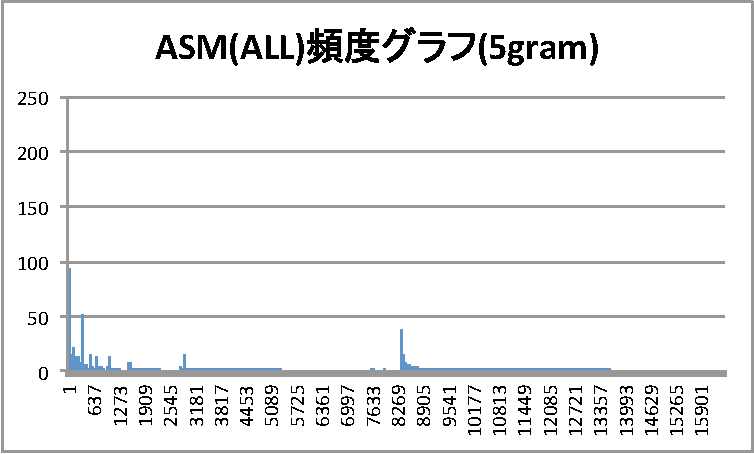
\includegraphics[clip,width=0.47\textwidth]{ALL}
  }
   \subfigure[Duplication registers]{
    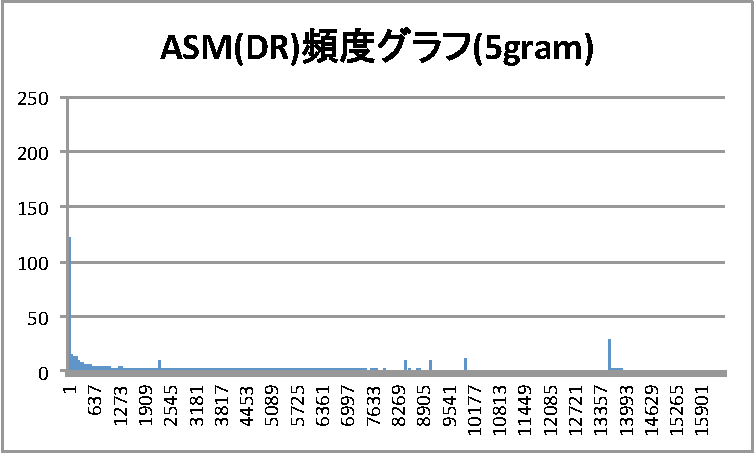
\includegraphics[clip,width=0.47\textwidth]{DR}
  }
 \subfigure[Irreducibility]{
    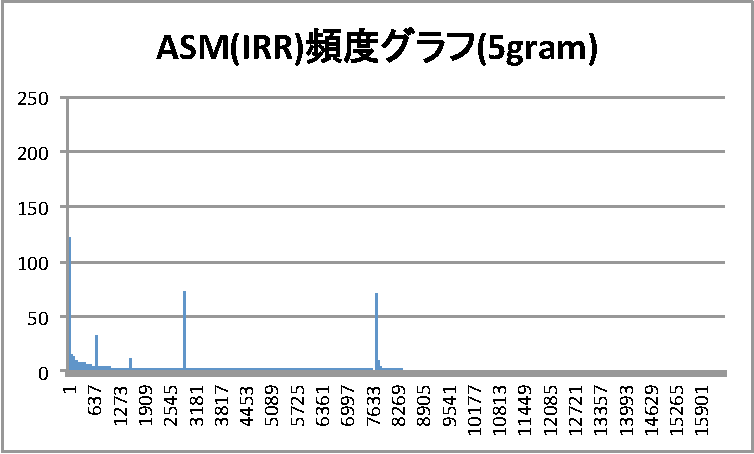
\includegraphics[clip,width=0.47\textwidth]{IRR}
  }
 \subfigure[Merge Local Integer]{
    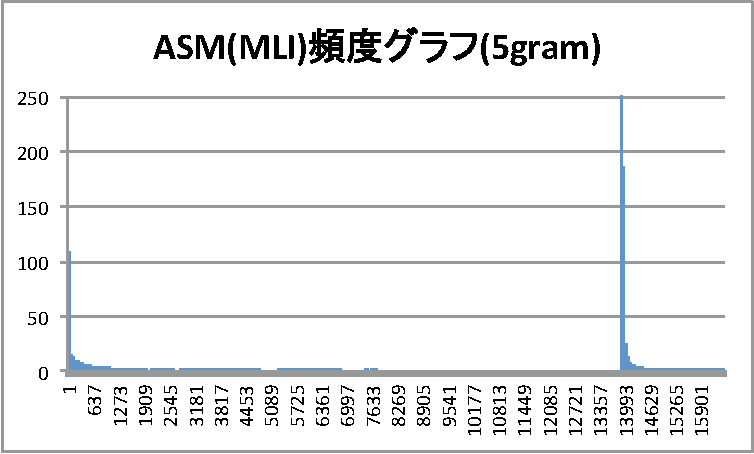
\includegraphics[clip,width=0.47\textwidth]{MLI}
  }
 \subfigure[ProGuard]{
    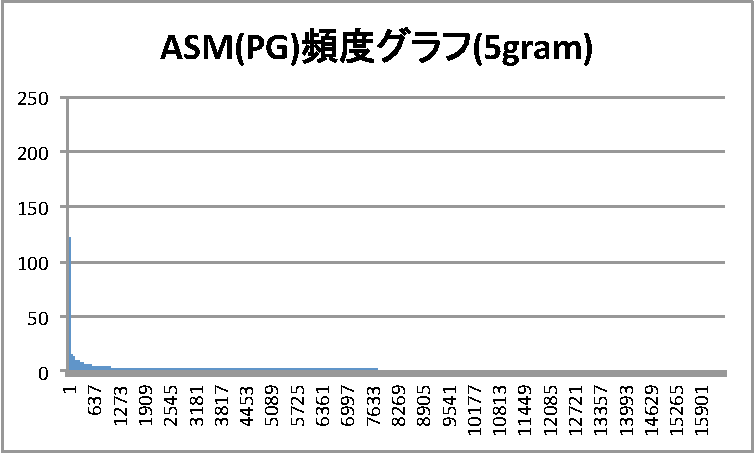
\includegraphics[clip,width=0.47\textwidth]{PG}
  }
  \caption{ASM(5gram)頻度のグラフ}\label{fig:graph}
\end{figure}


 \end{document}
